%
% Clasificación de cifrados de flujo, capítulo de antecedentes.
% Proyecto Lovelace.
%

\subsection{Clasificación}

Una clasificación común es en \textit{síncronos} y
en \textit{autosincronizables}. A continuación se describen a grandes rasgos
ambos modelos.

\subsubsection{Síncronos}

Un cifrado de flujo síncrono es aquel en el que el flujo de la llave es
generado de manera independiente del texto en claro y del texto cifrado. Se
puede definir un modelo general con las siguientes tres ecuaciones.
\begin{align}
  \label{sinc:cambio_de_estado}
  e_{i+1} &= f(e_i, K) \\
  \label{sinc:flujo_de_llave}
  k_i &= g(e_i, K) \\
  \label{sinc:funcion_de_salida}
  c_i &= h(k_i, m_i)
\end{align}
La letra $ e $ representa el estado del cifrado, $ K $ es la llave, $ k $ es
la salida del flujo de llave, $ c $ es el texto cifrado y $ m $ es el texto en
claro. La función de la ecuación \ref{sinc:cambio_de_estado} ($ f $) es la que
describe el cambio de estado; este se determina a partir del estado actual y
de la llave. En la ecuación \ref{sinc:flujo_de_llave} se describe la acción del
flujo de llave ($ g $): para determinar el próximo símbolo se emplea solamente
el estado actual y la llave. La tercera ecuación (\ref{sinc:funcion_de_salida},
$ h $) describe la acción de combinar el flujo de la llave con el mensaje, y
así obtener el texto cifrado.

En la figura \ref{flujo_sincrono} se describe de manera gráfica las operaciones
de cifrado y descifrado; estas guardan muchas similitudes con el modo de
operación \gls{gl:ofb} (sección \ref{sec:ofb}), con la única excepción de
que este trabaja con bloques del tamaño del cifrado subyacente. En otras
palabras, si se definiera el tamaño del bloque (y en consecuencia el tamaño del
\gls{gl:vector_de_inicializacion}) como 1, entonces \gls{gl:ofb} sería un
cifrado de flujo síncrono.

\begin{figure}
  \centering
  \begin{subfigure}{0.45\textwidth}
    \begin{center}
      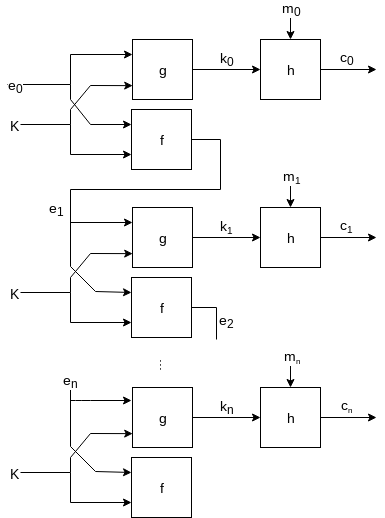
\includegraphics[width=0.9\linewidth]{diagramas/sincrono_cifrado.png}
      \caption{Cifrado.}
    \end{center}
  \end{subfigure}
  \begin{subfigure}{0.45\textwidth}
    \begin{center}
      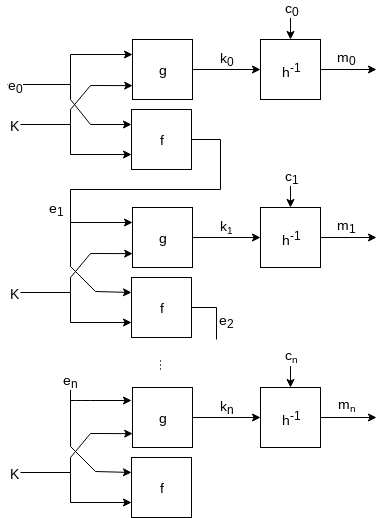
\includegraphics[width=0.9\linewidth]{diagramas/sincrono_descifrado.png}
      \caption{Descifrado.}
    \end{center}
  \end{subfigure}
  \caption{Esquema general de un cifrado de flujo síncrono.}
  \label{flujo_sincrono}
\end{figure}

El nombre de esta categoría proviene del hecho de que ambos entes del proceso
comunicativo (emisor y receptor) deben encontrarse sincronizados (usar la misma
llave y encontrarse en la misma posición) para que la comunicación tenga éxito:
si se insertan dígitos extras al mensaje cifrado, la sincronización se pierde.
Los cifrados de flujo síncronos no tienen propagación de error: aunque ciertos
bits sean modificados (pero no borrados) durante su transmisión, el resto del
mensaje sigue siendo descifrable.


\subsubsection{Autosincronizables}

En esta clasificación se engloban a aquellos cifrados cuyo flujo de llave es
resultado de la propia llave original y de cierto número previo de dígitos
cifrados. Las ecuaciones que describen su comportamiento son las siguientes.
\begin{align}
  \label{asinc:cambio_de_estado}
  e_{i+1} &= (c_{i - t}, c_{i - t + 1}, \dots, c_{i - 1}) \\
  \label{asinc:flujo_de_llave}
  k_i &= g(e_i, K) \\
  \label{asinc:funcion_de_salida}
  c_i &= h(k_i, m_i)
\end{align}
La notación es la misma que en las ecuaciones \ref{sinc:cambio_de_estado},
\ref{sinc:flujo_de_llave} y \ref{sinc:funcion_de_salida}. En este caso, el
próximo estado depende de $ t $ (el tamaño de la ventana) dígitos cifrados
anteriormente. En la figura \ref{flujo_asincrono} se describe de manera
gráfica el proceso de cifrado y descifrado.

\begin{figure}
  \centering
  \begin{subfigure}{0.45\textwidth}
    \begin{center}
      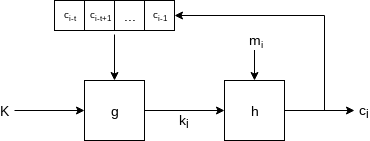
\includegraphics[width=0.9\linewidth]{diagramas/asincrono_cifrado.png}
      \caption{Cifrado.}
    \end{center}
  \end{subfigure}
  \begin{subfigure}{0.45\textwidth}
    \begin{center}
      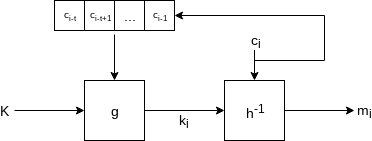
\includegraphics[width=0.9\linewidth]{diagramas/asincrono_descifrado.png}
      \caption{Descifrado.}
    \end{center}
  \end{subfigure}
  \caption{Esquema general de un cifrado de flujo autosincronizable.}
  \label{flujo_asincrono}
\end{figure}

En una antítesis de la categoría anterior, el nombre de esta indica que no es
necesario que el emisor y el receptor estén sincronizados: si se llegan a
perder bits en la transmisión, el esquema es capaz de autosincronizarse, pues
el flujo de la llave depende de cierto número de bits anteriores. A esta
categoría también se le conoce como «asíncrona».

La propagación de los errores depende del tamaño de ventana (el número $ t $
de bits previos utilizados para calcular la próxima llave), si se modifica un
bit, entonces los próximos $ t $ serán incorrectos.
